\chapter{A Probabilistic Approach to Grasp Synthesis}

\section{Introduction}

\section{Related work}

\section{Contributions}

\section{Probabilistic modelling of grasping success}
Grasp motion, is the key phase
in the entire grasping process. During this phase, the robot has to estimate the object pose and geometry, predict the likelihood of success with a pre-touch configuration and choose the action that maximizes the
grasping success probability. This sections gives the mathematic model of grasping success, followed by a the proof of the model with an 1-D grasping example. 
\subsection{Mathematic Model}
First we define a random variable $S \in \{ \text{success} , \text{failure} \}$ as the outcome of a specific grasp motion $\mathcal{G} = \{g_1, \dots ,g_n$\}, with $g_1, \dots ,g_n$ representing a set of gripper configurations and poses. We define $\text{P}({S = \text{success}}|\mathcal{G},\mathcal{Z})$ as the marginal probability that the grasp $\mathcal{G}$ succeeds based on the sensor measurement history $\mathcal{Z}=\lbrace z_0, \dots ,z_M \rbrace$. It is not straightforward to compute the marginal probability $\text{P}({S = \text{success}}|\mathcal{G},\mathcal{Z})$ directly without knowing the state of the object 
$x_o$. However, we can compute it by separating it into two probability terms: 
\begin{equation}
\text{P}(S) := \text{P}(S | \mathcal{G} ,\mathcal{Z}) = \int_{x_o} \text{P} (S | x_o,\mathcal{G} )\cdot p(x_o|\mathcal{Z}) dx_o. 
\label{e_grasp_success}
\end{equation}
We call the first term $P(S | x_o,\mathcal{G})$ conditional grasping success model. It indicates how likely a specific grasping action $\mathcal{G}$ will lead to a success given the object state $x_o$. The second term $p(x_o|\mathcal{Z})$ represents the posterior probability of the object given a series of observations, which quantifies the perception uncertainty. In this way, the problem of predicting the marginal grasp success probability is simplified to model the $P(S | x_o,\mathcal{G})$, and to model the perception uncertainty. 

After the marginal grasp probability $\text{P}(S)$ is computed, the next step is to find an optimal grasping motion $\mathcal{G}_\text{opt}$ that maximizes the marginal grasp success probability:
\begin{equation}
\mathcal{G}_\text{opt} = \argmax_\mathcal{G} \text{P}(S).
\label{eq_g_opt}
\end{equation}

\subsection{Verification of the concept}
To verify the proposed mathematic model, we apply this formulation to solve an 1-D grasping problem. We aim to compute the optimal pre-touch configuration for a simple parallel gripper to grasp an 1-D rigid  object with width $w$. $x$ defines the position of the object. The parallel gripper has a limited opening width constrained by $u_1 \in [0, u_{1}^{\text{max}}]$. $u_2$ defines the position of the gripper. We assume that the grasp motion $\mathcal{G}$ only contains one gripper configuration defined by $\{ (u_1,u_2) \}$. Fig.~\ref{fig:1D_simple} depicts this 1-D grasping example.

\begin{figure}[!htbp]
\centering
\def\svgwidth{0.8\linewidth}
%% Creator: Inkscape inkscape 0.48.4, www.inkscape.org
%% PDF/EPS/PS + LaTeX output extension by Johan Engelen, 2010
%% Accompanies image file '1dillustration.pdf' (pdf, eps, ps)
%%
%% To include the image in your LaTeX document, write
%%   \input{<filename>.pdf_tex}
%%  instead of
%%   \includegraphics{<filename>.pdf}
%% To scale the image, write
%%   \def\svgwidth{<desired width>}
%%   \input{<filename>.pdf_tex}
%%  instead of
%%   \includegraphics[width=<desired width>]{<filename>.pdf}
%%
%% Images with a different path to the parent latex file can
%% be accessed with the `import' package (which may need to be
%% installed) using
%%   \usepackage{import}
%% in the preamble, and then including the image with
%%   \import{<path to file>}{<filename>.pdf_tex}
%% Alternatively, one can specify
%%   \graphicspath{{<path to file>/}}
%% 
%% For more information, please see info/svg-inkscape on CTAN:
%%   http://tug.ctan.org/tex-archive/info/svg-inkscape
%%
\begingroup%
  \makeatletter%
  \providecommand\color[2][]{%
    \errmessage{(Inkscape) Color is used for the text in Inkscape, but the package 'color.sty' is not loaded}%
    \renewcommand\color[2][]{}%
  }%
  \providecommand\transparent[1]{%
    \errmessage{(Inkscape) Transparency is used (non-zero) for the text in Inkscape, but the package 'transparent.sty' is not loaded}%
    \renewcommand\transparent[1]{}%
  }%
  \providecommand\rotatebox[2]{#2}%
  \ifx\svgwidth\undefined%
    \setlength{\unitlength}{244.80062425bp}%
    \ifx\svgscale\undefined%
      \relax%
    \else%
      \setlength{\unitlength}{\unitlength * \real{\svgscale}}%
    \fi%
  \else%
    \setlength{\unitlength}{\svgwidth}%
  \fi%
  \global\let\svgwidth\undefined%
  \global\let\svgscale\undefined%
  \makeatother%
  \begin{picture}(1,0.30919334)%
    \put(0,0){\includegraphics[width=\unitlength]{1dillustration.pdf}}%
    \put(0.15949338,0.01813248){\color[rgb]{0,0,0}\makebox(0,0)[lb]{\smash{$u_2$}}}%
    \put(0.40692504,0.22646518){\color[rgb]{0,0,0}\makebox(0,0)[lb]{\smash{object}}}%
    \put(0.96767264,0.21229788){\color[rgb]{0,0,0}\makebox(0,0)[lb]{\smash{$x$}}}%
    \put(0.44163201,0.13862415){\color[rgb]{0,0,0}\makebox(0,0)[lb]{\smash{$w$}}}%
    \put(0.4455571,0.29089082){\color[rgb]{0,0,0}\makebox(0,0)[lb]{\smash{$u_1$}}}%
    \put(-0.00215418,0.21245965){\color[rgb]{0,0,0}\makebox(0,0)[lb]{\smash{0}}}%
  \end{picture}%
\endgroup%

\captionsetup{justification=raggedright}
\caption{Illustration of an 1-D grasping problem.}
\label{fig:1D_simple}
\end{figure}	

First let us  derive a grasp success probability model $\text{P}(S | x,  \mathcal{G} )$ for this example. Since the positions of the finger tips can determine whether a gripper configuration will succeed, we can compute these positions directly from $u_1$ and $u_2$ by   

%It is obviously that when the  position of the gripper is equal to the position of the object ($u_2 = x$) and the opening width of the gripper is equal to the width of the object ($u_1 = w$), a stable grasp is then established. We define this configuration as a reference $u^{\text{ref}}$: 
%\begin{equation}
%u^{\text{ref}} =  \begin{pmatrix}\begin{figure}
%u_1^{\text{ref}}\\ 
%u_2^{\text{ref}}
%\end{pmatrix}
%=\begin{pmatrix}
%w\\ 
%x
%\end{pmatrix}. 
%\end{equation}
%and assign the probability of grasp success of this configuration with $\text{P}(S | x = x_0, \mathcal{G} = u^{\text{ref}}) = 1$.
\begin{equation}
\begin{pmatrix}
c^{\text{left}}\\ 
c^{\text{right}}
\end{pmatrix}
=\begin{pmatrix}
u_2 - 0.5 \cdot u_1\\ 
u_2 + 0.5 \cdot u_1
\end{pmatrix}.
\end{equation}
If the finger tips are in intersect with the object, the grasp is invalid. In these cases, we assign the probability of grasp success to zero. When the positions of finger tips fullfill the condition ( $c^{\text{left}} < x - 0.5w$ and $c^{\text{right}} > x + 0.5w$ ), the object can be grasped by the gripper. However, for precision grasping, we want to avoid object displacement during grasping. During the phase of force closure, we want the object to move as little as possible. Therefore, a term that penalizes object displacement can be introduced into the grasp success model. We model the grasp success probability by 

\begin{equation}
  \text{P}(S | x,  \mathcal{G} )  = -\frac{1}{ d^{\text{max}} } \cdot d + 1,
  \label{equ:5}
\end{equation}
where $d^{\text{max}}  = 0.5 \cdot (u_{1}^{\text{max}} - w) $ denotes the maximum displacement that can be executed by a gripper. $d = | u_2 - x | $ denotes the actual object displacement. By combining this model with a given object posterior $p(x|\mathcal{Z})$, a marginal success probability $\text{P}(S)$ can be obtained by evaluating Eq.~\ref{e_grasp_success}. To illustrate how an object posterior can influence marginal success probability, we choose object length $w = 0.2$, the maximal opening width of the gripper $u_{1}^{\text{max}} = 0.4 $. We compare the result by using two different object posteriors to simulate an accurate and a less accurate perception system. We model the $p(x|\mathcal{Z})$ by two Gaussian distributions with $\mathcal{N}(0, 0.3)$ and $\mathcal{N}(0, 0.03)$ respectively. Fig.~\ref{fig:1D_grasp} depicts the contour of grasp success probability $\text{P}(S)$ in terms of the pre-touch configuration.

\begin{figure}[!htbp]
\centering
\def\svgwidth{1\linewidth}
%% Creator: Inkscape inkscape 0.48.4, www.inkscape.org
%% PDF/EPS/PS + LaTeX output extension by Johan Engelen, 2010
%% Accompanies image file '1dgrasp_result.pdf' (pdf, eps, ps)
%%
%% To include the image in your LaTeX document, write
%%   \input{<filename>.pdf_tex}
%%  instead of
%%   \includegraphics{<filename>.pdf}
%% To scale the image, write
%%   \def\svgwidth{<desired width>}
%%   \input{<filename>.pdf_tex}
%%  instead of
%%   \includegraphics[width=<desired width>]{<filename>.pdf}
%%
%% Images with a different path to the parent latex file can
%% be accessed with the `import' package (which may need to be
%% installed) using
%%   \usepackage{import}
%% in the preamble, and then including the image with
%%   \import{<path to file>}{<filename>.pdf_tex}
%% Alternatively, one can specify
%%   \graphicspath{{<path to file>/}}
%% 
%% For more information, please see info/svg-inkscape on CTAN:
%%   http://tug.ctan.org/tex-archive/info/svg-inkscape
%%
\begingroup%
  \makeatletter%
  \providecommand\color[2][]{%
    \errmessage{(Inkscape) Color is used for the text in Inkscape, but the package 'color.sty' is not loaded}%
    \renewcommand\color[2][]{}%
  }%
  \providecommand\transparent[1]{%
    \errmessage{(Inkscape) Transparency is used (non-zero) for the text in Inkscape, but the package 'transparent.sty' is not loaded}%
    \renewcommand\transparent[1]{}%
  }%
  \providecommand\rotatebox[2]{#2}%
  \ifx\svgwidth\undefined%
    \setlength{\unitlength}{259.88395945bp}%
    \ifx\svgscale\undefined%
      \relax%
    \else%
      \setlength{\unitlength}{\unitlength * \real{\svgscale}}%
    \fi%
  \else%
    \setlength{\unitlength}{\svgwidth}%
  \fi%
  \global\let\svgwidth\undefined%
  \global\let\svgscale\undefined%
  \makeatother%
  \begin{picture}(1,0.53724423)%
    \put(0,0){\includegraphics[width=\unitlength]{1dgrasp_result.pdf}}%
    \put(0.1151589,0.08992018){\makebox(0,0)[lb]{\smash{0.2}}}%
    \put(0.18217497,0.08992018){\makebox(0,0)[lb]{\smash{0.25}}}%
    \put(0.27003572,0.08992018){\makebox(0,0)[lb]{\smash{0.3}}}%
    \put(0.33673164,0.08992018){\makebox(0,0)[lb]{\smash{0.35}}}%
    \put(0.4249133,0.08992018){\makebox(0,0)[lb]{\smash{0.4}}}%
    \put(0.08972926,0.1171398){\makebox(0,0)[lb]{\smash{-0.5}}}%
    \put(0.07593948,0.20747584){\color[rgb]{0,0,0}\makebox(0,0)[lb]{\smash{-0.25}}}%
    \put(0.10355064,0.2982193){\makebox(0,0)[lb]{\smash{0}}}%
    \put(0.08669901,0.39782419){\makebox(0,0)[lb]{\smash{0.25}}}%
    \put(0.09666237,0.48644253){\makebox(0,0)[lb]{\smash{0.5}}}%
    \put(0.23790599,0.1699559){\rotatebox{-22.99998994}{\makebox(0,0)[lb]{\smash{0.04}}}}%
    \put(0.27574288,0.23088155){\rotatebox{-25.9999936}{\makebox(0,0)[lb]{\smash{0.08}}}}%
    \put(0.33923275,0.31457275){\rotatebox{-51.0000188}{\makebox(0,0)[lb]{\smash{0.12}}}}%
    \put(0.01695468,0.30375214){\color[rgb]{0,0,0}\makebox(0,0)[lb]{\smash{$u_2$}}}%
    \put(0.27728722,0.04517519){\color[rgb]{0,0,0}\makebox(0,0)[lb]{\smash{$u_1$}}}%
    \put(0.61970258,0.09198088){\makebox(0,0)[lb]{\smash{0.2}}}%
    \put(0.68671864,0.09198088){\makebox(0,0)[lb]{\smash{0.25}}}%
    \put(0.77457939,0.09198088){\makebox(0,0)[lb]{\smash{0.3}}}%
    \put(0.84127531,0.09198088){\makebox(0,0)[lb]{\smash{0.35}}}%
    \put(0.92945698,0.09198088){\makebox(0,0)[lb]{\smash{0.4}}}%
    \put(0.83165564,0.29547016){\rotatebox{-3.00000411}{\makebox(0,0)[lb]{\smash{0.7}}}}%
    \put(0.52418668,0.30637183){\color[rgb]{0,0,0}\makebox(0,0)[lb]{\smash{$u_2$}}}%
    \put(0.7845194,0.05087321){\color[rgb]{0,0,0}\makebox(0,0)[lb]{\smash{$u_1$}}}%
    \put(0.26204153,0.00490434){\color[rgb]{0,0,0}\makebox(0,0)[lb]{\smash{(a)}}}%
    \put(0.79104124,0.0040583){\color[rgb]{0,0,0}\makebox(0,0)[lb]{\smash{(b)}}}%
    \put(0.58730417,0.21390265){\color[rgb]{0,0,0}\makebox(0,0)[lb]{\smash{-0.25}}}%
    \put(0.59889533,0.11916901){\makebox(0,0)[lb]{\smash{-0.5}}}%
    \put(0.61271672,0.30024851){\makebox(0,0)[lb]{\smash{0}}}%
    \put(0.59586509,0.3998534){\makebox(0,0)[lb]{\smash{0.25}}}%
    \put(0.60582844,0.48847175){\makebox(0,0)[lb]{\smash{0.5}}}%
  \end{picture}%
\endgroup%

\caption{ Marginal grasp success probability in terms of two different object posteriors. The optimal gripper configurations are shown by red dots. In (a), $\mathcal{N}(0, 0.3)$ is used to simulate the posterior of the object position. The marginal success probability ${\text{P}(S)}_{u = u_{\text{opt}}} = 0.13$  . In (b) $\mathcal{N}(0, 0.03)$ is used to simulate a more accurate posterior distribution of the object position with ${\text{P}(S)}_{u = u_{\text{opt}}} = 0.76$ }
\label{fig:1D_grasp}
\end{figure}	 


\subsection{Modelling of conditional grasp success probability }
For real world objects, it is required to have a conditional grasp success model that consider much more factors than the 1-D example, so that the conditional grasp success model can approximate the true probability. Two conditions are necessary to ensure a successful grasp. First, the motion of a gripper, which is represented by $\mathcal{G}$, should not collide with the environment and the object. Second, the last pose and posture $g_n$ which we define as the pre-touch configuration should guarantee that forces from the finger tips are established on the object in the third phase. For the first condition we assume that there is sufficient free space between the pre-grasp configuration and the pre-touch configuration. The collision-free motion from the pre-grasp to the pre-touch can be computed using a pre-defined heuristic: approaching with a linear motion. To fullfill the second condition, the choice of a pre-touch configuration $g_n$ is essential, because the grasp success is predominantly affected by the way we make contact with the object. Hence, the grasp success model $P(S | x,\mathcal{G})$ is simplified to $P(S | x, g_n$). 

The dimension of the object state $x$ depends on the choice of an object representation. To represent simple geometry primitives such as cylindrical objects, it is sufficient to choose a parametric representation which includes radius, height, and the position of the object. For objects which form are irregular, the dimension of $x$ can be very large. However, predicting the grasp success probability can be independent of the choice of representation, since it is only required to extract the contact normals of an object.  

In the following we elaborate on how we calculate the conditional success probability of a pre-touch configuration $g_n$ for real world objects. Here we only study the pinch grasp, that a grasp only requires two fingers to make contact with the object. Pinch grasp can be easily realized by most grippers, independent of how many fingers a gripper having. We choose three criteria to model the conditional grasp success probability. 

\begin{figure}[!htbp]
\centering
\def\svgwidth{0.7\linewidth}
%% Creator: Inkscape inkscape 0.48.4, www.inkscape.org
%% PDF/EPS/PS + LaTeX output extension by Johan Engelen, 2010
%% Accompanies image file 'bunny.pdf' (pdf, eps, ps)
%%
%% To include the image in your LaTeX document, write
%%   \input{<filename>.pdf_tex}
%%  instead of
%%   \includegraphics{<filename>.pdf}
%% To scale the image, write
%%   \def\svgwidth{<desired width>}
%%   \input{<filename>.pdf_tex}
%%  instead of
%%   \includegraphics[width=<desired width>]{<filename>.pdf}
%%
%% Images with a different path to the parent latex file can
%% be accessed with the `import' package (which may need to be
%% installed) using
%%   \usepackage{import}
%% in the preamble, and then including the image with
%%   \import{<path to file>}{<filename>.pdf_tex}
%% Alternatively, one can specify
%%   \graphicspath{{<path to file>/}}
%% 
%% For more information, please see info/svg-inkscape on CTAN:
%%   http://tug.ctan.org/tex-archive/info/svg-inkscape
%%
\begingroup%
  \makeatletter%
  \providecommand\color[2][]{%
    \errmessage{(Inkscape) Color is used for the text in Inkscape, but the package 'color.sty' is not loaded}%
    \renewcommand\color[2][]{}%
  }%
  \providecommand\transparent[1]{%
    \errmessage{(Inkscape) Transparency is used (non-zero) for the text in Inkscape, but the package 'transparent.sty' is not loaded}%
    \renewcommand\transparent[1]{}%
  }%
  \providecommand\rotatebox[2]{#2}%
  \ifx\svgwidth\undefined%
    \setlength{\unitlength}{194bp}%
    \ifx\svgscale\undefined%
      \relax%
    \else%
      \setlength{\unitlength}{\unitlength * \real{\svgscale}}%
    \fi%
  \else%
    \setlength{\unitlength}{\svgwidth}%
  \fi%
  \global\let\svgwidth\undefined%
  \global\let\svgscale\undefined%
  \makeatother%
  \begin{picture}(1,0.67409794)%
    \put(0,0){\includegraphics[width=\unitlength]{bunny.pdf}}%
    \put(0.12693299,0.16410315){\color[rgb]{0,0,0}\makebox(0,0)[lb]{\smash{$n_1$}}}%
    \put(0.7863913,0.49764194){\color[rgb]{0,0,0}\makebox(0,0)[lb]{\smash{$n_2$}}}%
    \put(0.64071158,0.3573397){\color[rgb]{0,0,0}\makebox(0,0)[lb]{\smash{$c_2$}}}%
    \put(0.31678681,0.21094795){\color[rgb]{0,0,0}\makebox(0,0)[lb]{\smash{$c_1$}}}%
    \put(0.19497423,0.18987635){\color[rgb]{0,0,0}\makebox(0,0)[lb]{\smash{$d_1$}}}%
    \put(0.76565879,0.40945617){\color[rgb]{0,0,0}\makebox(0,0)[lb]{\smash{$d_2$}}}%
  \end{picture}%
\endgroup%

\caption{Description of variables which represent a pre-touch configuration $g_n$ on an bunny object. Fingertips are illustrated in blue. Dashed lines indicate variances of the representation. Arrows represent normals on the particular surfaces.}
\label{fig:grasp_generation}
\end{figure}

\begin{itemize}
\item \textit{Non-zero contact angle}: 
 The first criterion that affects the grasp success is the angle between normal of finger tips and desired contact regions. In Fig.~\ref{fig:grasp_generation}, we denote $n_i$ as the normal defined on a finger tip and $c_i$ as the normal of a contact region. $d_i$ is the distance from a finger tip to a contact region. The grasp success probability with a non-zero contact angle is given by:
\begin{equation}
P_1 = \begin{cases}
\prod_{i=1}^{k}(-\frac{1}{0.5\cdot \theta} |\beta|) + 1 )  & |\beta | < \frac{\theta}{2}\\
  0   & \text{else}
\end{cases},
\end{equation} 
where $\beta = \pi - \angle(n_i,c_i)$ and $\angle(n_i,c_i)$ is the angle between $n_i$ and $c_i$.  $k$ denotes the total number of finger tips used to make contact with the object. $\theta$ is the maximal angle of a friction cone that the finger tip still supports the object without slipping. 
\item \textit{Non-optimal finger placement}:
Due to the non-optimal control of a gripper during force closure, the closer the finger tips are located to the object surface, the less likely a control error would occur to influence the overall grasp success. Therefore this criterion is modelled by 
\begin{equation} 
P_2 = \text{exp}\left(-\sum_{i=1}^k \frac{d_i-h}{\sigma_h^2}\right)
\end{equation}
where $h$ is the desired offset distance between finger tips and the object's surface for a pre-touch configuration. $\sigma_h$ is a shaping factor for the probability. 

\todo {\item \textit{Distance to center of gravity}:}
 

\item \textit{Surface uncertainty}:
 This criterion is specially designed for the representation that is able to model surface uncertainty. This criterion avoids to make finger contacts on uncertain surfaces, because contacts established on uncertain surfaces can not guarantee firm contacts between the finger tips and the object. We model the success probability of uncertain contacts induced by surface uncertainty with 
\begin{equation}
 P_3 =  \begin{cases}
\prod_{i=1}^{k}(-\frac{1}{\sigma_{\text{max}} } \mean{\sigma(c_i)}  + 1 )  &  \mean{\sigma(c_i)} < \sigma_{\text{max}}\\
  0   & \text{else}
\end{cases},
\end{equation} 
where $\mean{\sigma(c_i)} $ is an average variance of $c_i$ and $\sigma_{\text{max}}$ is a parameter representing the maximal allowed variance. We merge the proposed  criteria in a weighted fashion to generate an overall grasp success probability by  
\begin{equation}
P(S | x , g_n) =  \sum_{i=1}^3 w_i \cdot P_i
\end{equation} 
with $\sum_{i=1}^3 w_i  = 1$.
\end{itemize}

\subsection{Model validation}
We choose a 2-D grasp scenario to validate the model of  conditional grasp success probability. A circular object is chosen as the target object. The circular object is represented by three parameters: radius $\in \mathcal{R}$ and position $\in \mathcal{R}^2$. A parallel gripper is chose to grasp the object. The gripper configuration $\in \mathcal{R}^4$ contains the 2D positions of the left finger and the right finger. We simplify the grasp trajectory $\mathcal{G}$ to $g_n$, which is by definition the pre-touch configuration.  A number of random gripper pre-touch configurations is generated. For each configuration we evaluate the conditional grasp success probability. Fig.~\ref{fig:circular_grasp_success}(a) depicts 10 random gripper configurations, the grasp success probability of which are higher than 90~$\%$. Fig.~\ref{fig:circular_grasp_success}(b) shows 10 negative examples, the conditional grasp success probability of which are lower than 10~$\%$. 

The optimal pre-touch configuration is found according to equation \ref{eq_g_opt} by searching the maximal marginal grasp probability. Since the dimension of object state for a circular object is only three, we can integrate the equation \ref{e_grasp_success} numerically. Suppose the posterior of the object state can be represented by a multi-variate Gaussian $p(x_o|\mathcal{Z}) = \mathcal{N}(\mu, \Sigma)$ where $\mu$ is a mean and $\Sigma$ is a covariance matrix. The integral of equation  \ref{e_grasp_success} can be approximated by 

\begin{equation}
\begin{split}
 \text{P}(S | \mathcal{G} ,\mathcal{Z}) &= \text{P}(S | g_n ,\mathcal{Z}) \\
    &= \int_{x_o} \text{P} (S | x_o, g_n )\cdot p(x_o|\mathcal{Z}) dx_o \\
    &=  \int_{x_o} \text{P} (S | x_o, g_n )\cdot \mathcal{N}(\mu, \Sigma) dx_o  \\
    &\approx \int_{\mu_1 - \sigma_1}^{\mu_1 + \sigma_1} \int_{\mu_2 - \sigma_2}^{\mu_2 + \sigma_2} \int_{\mu_3 - \sigma_3}^{\mu_3 + \sigma_3} \text{P} (S | x_{o},  g_n )\cdot \mathcal{N}(\mu, \Sigma)  dx_{1} dx_{2} dx_{3}, 
\label{e_grasp_success}
\end{split}
\end{equation}
where $x_{1}, x_{2}, x_{3} $ represent the radius and the positions, $\mu_1, \mu_2, \mu_3$ are the means of positions and the radius. $\sigma_1, \sigma_2, \sigma_3$ are the diagonal elements of the covariance matrix $\Sigma$. In this case, we use Subplex \todo{[cite]\cite{}}(a variant of Nelder-Mead for function minimization) implemented in NLopt \todo{[cite]\cite{}} to find the maximal probability of $\text{P}(S | g_n ,\mathcal{Z})$. Fig.~\ref{fig:object_posterior_sample} visualizes a synthetic posterior distribution   with $\mu = (0, 0 , 0.01)$ and $
\Sigma = 
\begin{pmatrix}
0.01 & 0.008  & 0 \\ 
0.008 & 0.01  & 0 \\
0 & 0  & 0.01
\end{pmatrix}
$. The optimal pre-touch configuration for this posterior is depicted in Fig.~\ref{fig:optimal_pre_touch_conf}. The marginal success probability of this object posterior by taking the optimal pre-touch configuration is equal to $44.9 \%$. The absolute mass of probability depends on how the parameters are chosen for evaluating the conditional success grasp probability. Since the parameters we choose for calculating the conditional success grasp probability for this example is conservative, the success probability by taking the optimal pre-touch configuration is not high. However, the pre-touch configurations computed using our model are very close to the optimal in reality. From the figure we can see, that the grasp is explicitly computed for the given object state uncertainty. 

\begin{figure}[!htbp]
\centering
\def\svgwidth{1\linewidth}
\input{figure/grasp_success_circular.tex}
\caption{Ten random sampled good (a) $P(S | x ,g_n) > 0.9$ and bad (b) pre-touch configurations $P(S |x,g_n) < 0.1$ evaluated with the proposed model.}
\label{fig:circular_grasp_success}
\end{figure}	 

\begin{figure}
    \centering
    \begin{subfigure}[b]{0.45\textwidth}
        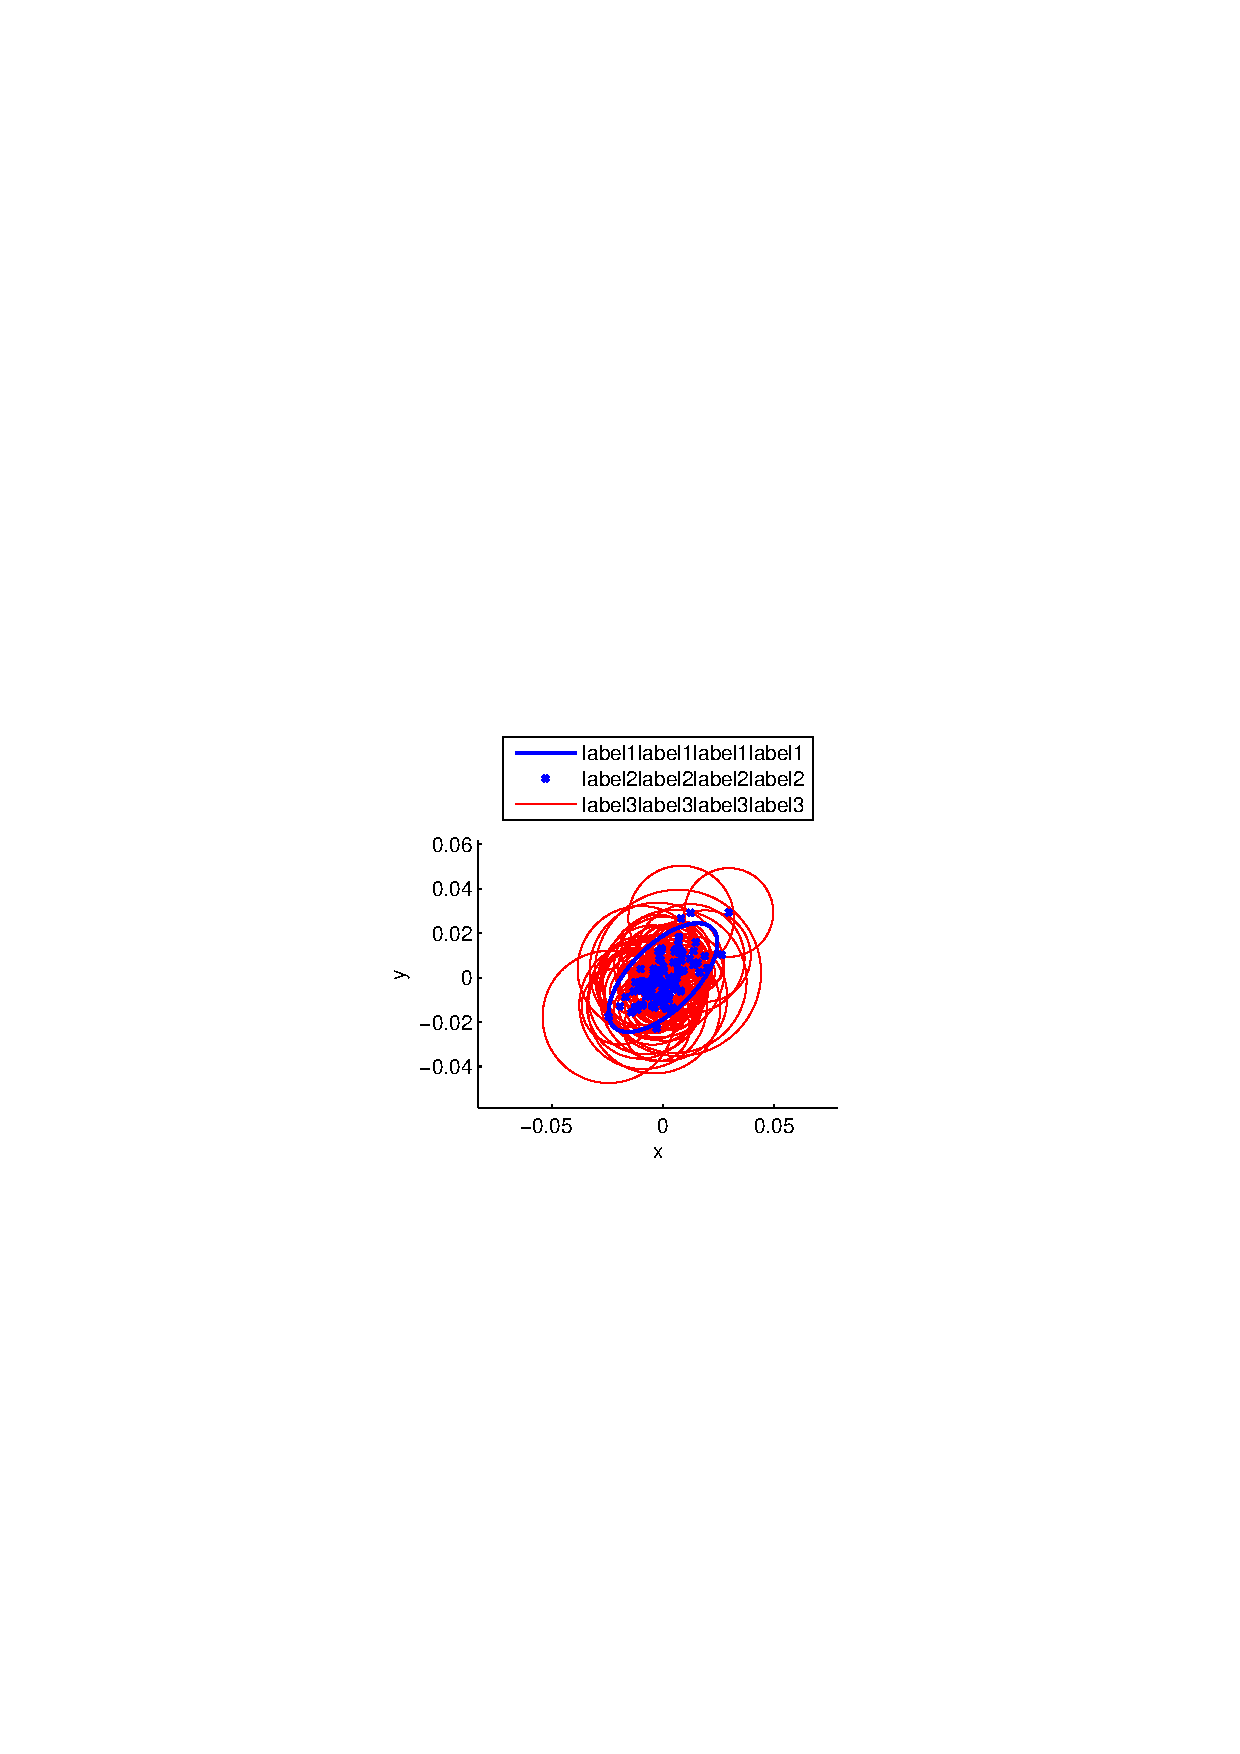
\includegraphics[width=\textwidth]{object_posterior_sample.pdf}
        \caption{A synthetic object posterior $p(x_o|\mathcal{Z} = \mathcal{N}(\mu, \Sigma)$ where $\mu = \left( 0.01,0,0  \right) $ and $\Sigma$ is a covariance matrix with $\sigma_x = \sigma_y = \sigma_r = 0.01$ , $\sigma_{xy} = 0.008$ and $\sigma_{rx} = \sigma_{ry} = 0$ }
        \label{fig:object_posterior_sample}
    \end{subfigure}
    ~ %add desired spacing between images, e. g. ~, \quad, \qquad, \hfill etc. 
      %(or a blank line to force the subfigure onto a new line)
    \begin{subfigure}[b]{0.45\textwidth}
        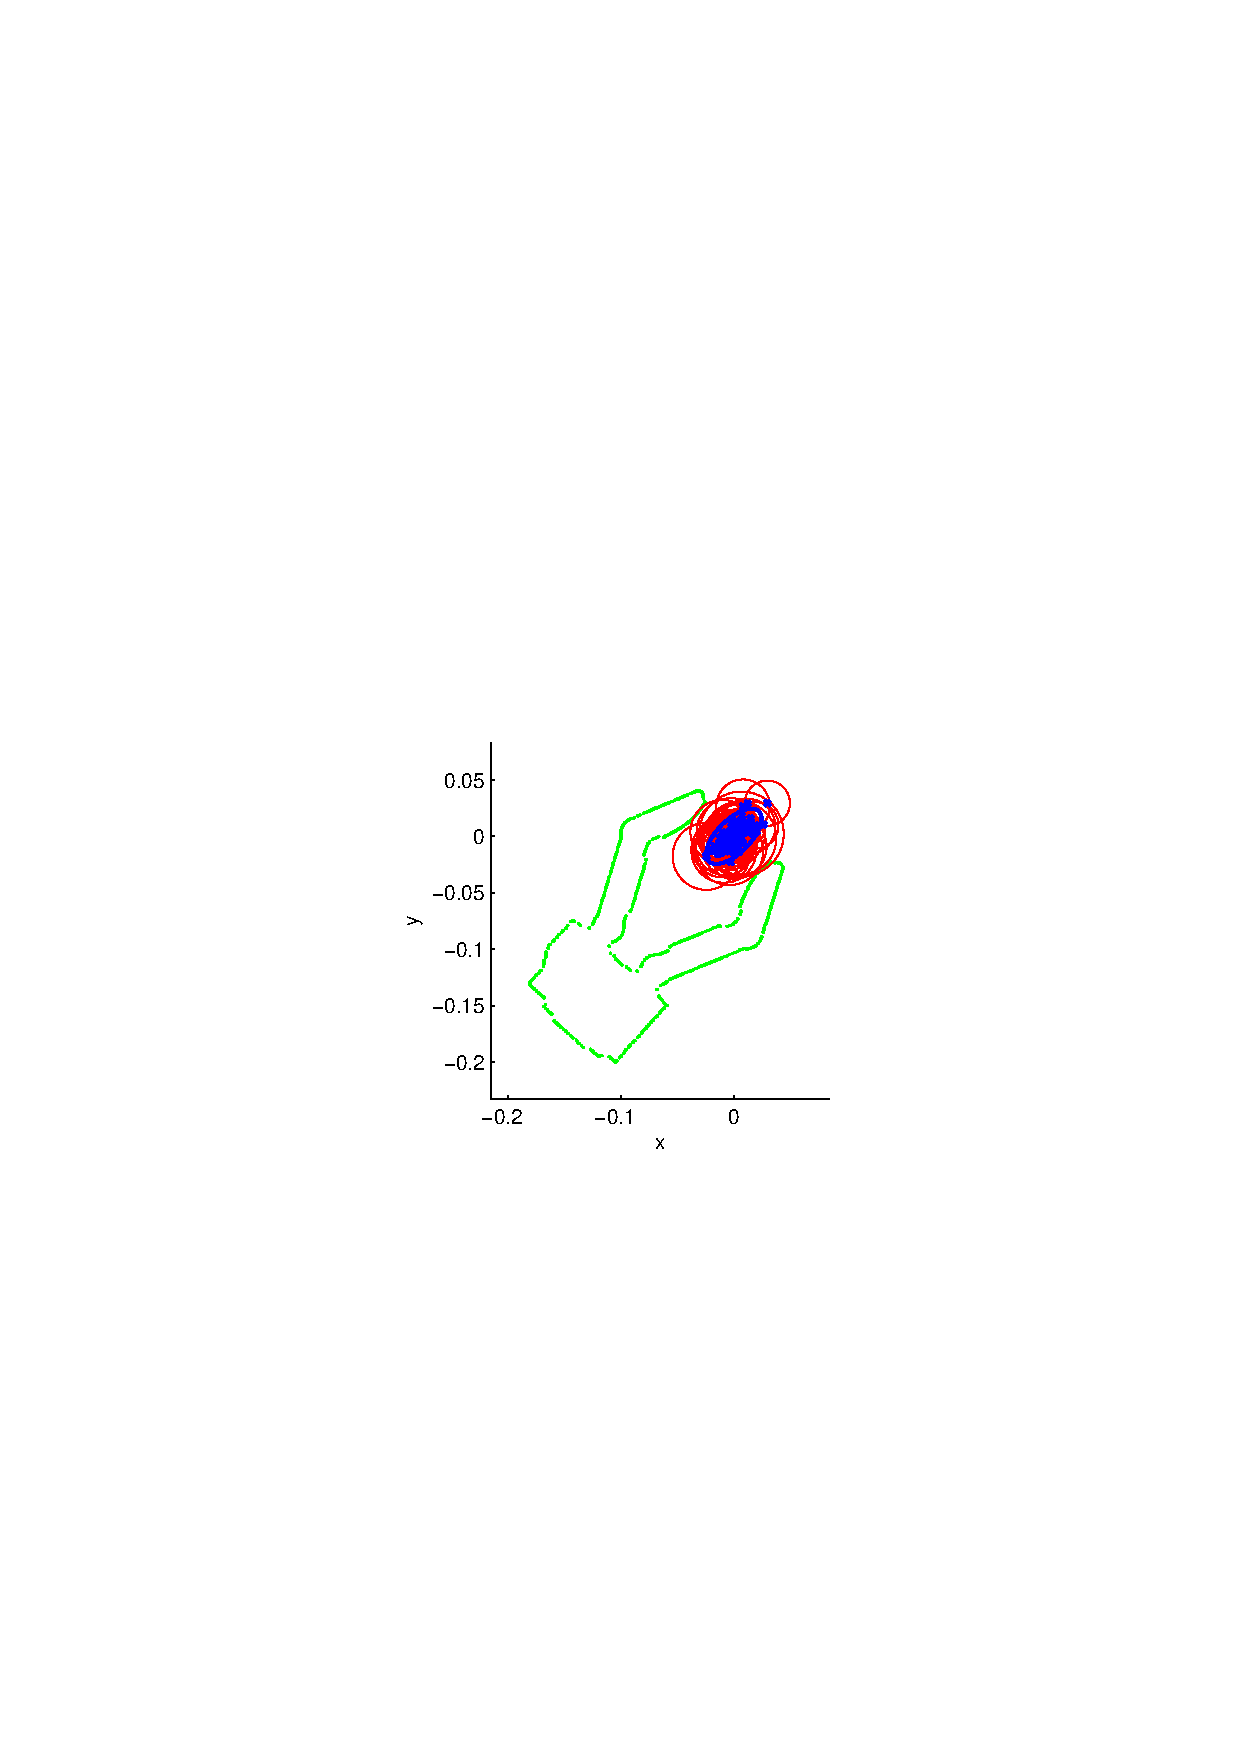
\includegraphics[width=\textwidth]{optimal_pre_touch_conf.pdf}
        \caption{The optimal pre-touch configuration computed for a circular object with the posterior shown to the left. The marginal success probability is $\text{P}(S) = 0.449$.}
        \label{fig:optimal_pre_touch_conf}
    \end{subfigure}
    \caption{An optimal pre-touch configuration computed for a given multivariate Gaussian posterior.}\label{fig:2dexample}
\end{figure}










\section{Modelling perception uncertainty}

%\subsection{Shape-primitive based probability distribution estimation using extended Kalman filter}


\subsection{Surface based probability distribution estimation based on probabilistic fusion}
The aforementioned shape-based approach that aim to represent the object with a limited number of parameter does not scale to real world objects. The reason is that the shapes and surfaces of most real world objects are complex and individual. Grasping these objects requires a robot to have the capability of learning the shape of irregular objects online even the object is presented for the first time. In this section we propose a new method to estimate the probability distribution of the surface of the objects. Rather than predict the shape parameter, this method estimate the course of the object surface achieved by a new probabilistic object representation and a multi-sensor fusion approach. Our surface representation has some significant advantages. First, it models the measurement uncertainty explicitly, as the fusion method explicitly takes Second, the model can be reconstructed with multiple measurements generated by multiple sensors, which have different noise characteristics. Third, one can parallelize the fusion method on GPU, so that the reconstruction
process is performed in real time. Fourth, the efficient query of the surface information allows fast grasp synthesis.

\subsection{Surface representation: p-SDF}
The model of the surface representation is based on signed distance field (SDF). A SDF in a metric space determine the distance between a point and the object surface. The sign of the distance indicates whether the point is outside or inside the object. Besides the distance information we augment the SDF with another additional variable $\sigma$ to represent the uncertainty of the distance. We call this new probabilistic surface representation p-SDF. In this work, a discretized version of p-SDF is used. We discretize a predefined metric space, where p-SDF is defined, into equally sized voxels. We denote the set of all the voxels as $V$. Since the modelling of an object can never be perfect, we have to take the surface uncertainty of modelling into account. To explicitly model the surface uncertainty, we define the distance to each voxel as a normal-distributed random variable. Thus, an object is represented by  
\begin{equation}
\bm{f}: v \mapsto \mathcal{N}(\mu, \sigma^2),  \forall v \in  V ,
\end{equation}
where $\mu$ is the mean and $\sigma$ is the variance of the distribution assigned to voxel $v$.  

\subsection{Surface reconstruction with sensor fusion}
In order to fuse the measurements into the representation using multiple sensors, an iterative method is used to update all the voxel elements. Considering only one voxel $v\in V$, we introduce a  random variables $D_{k}$ associated with voxel $v$. Here, $k$ denotes a time stamp. $\text{Bel}(D_{k-1})$ and $\text{Bel}(D_{k})$ represent the belief signed distance distributions at time stamp $k-1$ and $k$ respectively. We also assume that the major error of one sensor measurement can be approximated as Gaussian white noise, so we can define a measurement model of the sensor by
\begin{equation}
\text{P}(z|c,\Omega) = \mathcal{N}(z^*,  \sigma_\text{sensor}^2), 
\end{equation}
where $c$ denotes a depth camera pose and $\Omega$ denotes the surface of an object. $z^*$ is the true distance between the surface and the depth camera. Furthermore, we denote the true distance between the voxel $v$ to the surface $\Omega$ as $z_\text{sdf}^*$. From Fig.~\ref{fig:sdf} we can derive 
\begin{equation}
z_\text{sdf}^*  = d_{( v,c) } - z^*
\end{equation}
where $d_{( v,c) }$ denotes the distance between the voxel $v$ and the depth camera. Since $z$ follows a Gaussian distribution, $z_\text{sdf}$ also follows a Gaussian distribution, which is given by 
\begin{equation}
\text{P}(z_\text{sdf}|c,\Omega) = \mathcal{N}(z_\text{sdf}^*,  \sigma_\text{sensor}^2).
\end{equation}

\begin{figure}[!htbp]
\centering
\def\svgwidth{0.8\linewidth}
\input{figure/sdf.tex}
\caption{Description of the variables that we defined. The grid denotes the volume we consider for modelling an object. $z^*$ is the true measurement from a depth camera. $c$ denotes the pose of the depth camera. $ z_\text{sdf}^*$ is the true signed distance along the direction of the measurement.}
\label{fig:sdf}
\end{figure}	

The belief distribution  $\text{Bel}(D_{k})$ of voxel $v$ can be derived by Bayesian recursive updating by   


\begin{equation}
\begin{split}
\text{Bel}(D_{k}) &= \text{P}(D_{k} | z_\text{sdf}^1,\cdots, z_\text{sdf}^k) \\
                  &= \eta \cdot \text{P}(z_\text{sdf}^k | D_{k} ) \cdot  \text{P}(D_{k-1}|z_\text{sdf}^1\cdots z_\text{sdf}^{k-1} )  \\
                  &= \eta \cdot \text{P}(z_\text{sdf}^k | D_{k} ) \cdot \text{Bel}(D_{k-1})
  \end{split}
\end{equation}   
This equation shows that $\text{Bel}(D_{k})$ can be computed iteratively by the measurement model and the belief prior to the measurement update. In this work, we propose to approximate the belief with a Gaussian distribution for each voxel, so the belief  $\text{Bel}(D_{k})$ can be further computed by 

\begin{equation}
\begin{split}
\text{Bel}(D_{k}) &= \eta \cdot \mathcal{N}(z_\text{sdf},  \sigma_\text{sensor}^2) \cdot  \mathcal{N}( \mu_{k-1} ,   \sigma_{k-1} ^2) \\
&= \eta' \cdot \mathcal{N}( \mu_{k} ,   \sigma_{k} ^2)
  \end{split}
\end{equation}   

with 

\begin{equation}
\label{equ:rule1}
\begin{split}
  {\mu}_{k} &= \frac{{\mu}_{k-1}\cdot\sigma_\text{sensor}^{2}+  z_\text{sdf} \cdot\sigma_{k-1}^{2}}{\sigma_{k-1}^{2}+\sigma_\text{sensor}^2}
\end{split}
\end{equation}
%
\begin{equation}
\label{equ:rule2}
\begin{split}
  \sigma_{k}^{2} &=\frac{\sigma_{k-1}^{2}\cdot\sigma_\text{sensor}^2}{\sigma_{k-1}^{2}+\sigma_\text{sensor}^2}.
\end{split}
\end{equation}
We use Equ.~\ref{equ:rule1} and Equ.~\ref{equ:rule2} to update the whole volume $V$. To update the volume with another depth camera, one only needs to exchange $\sigma_\text{sensor}^2$ to the variance which represents the measurement characteristics of the camera. 



\section{Searching for feasible grasp configuration}

In general, numerous pre-touch configurations are feasible for a successful grasp, since most objects can be stably grasped in different ways. The marginal probability $P(s|g_n,\bm{f})$ is a high-dimensional non-convex function with respect to $g_n$. $g_n$ is parameterized by the pose of the gripper relatively to the object and the positions of joints. Finding the optimum of $g_n$ is not trivial. We propose to solve this problem in two steps. First, we use a generalizable method to parametrize the grasp posture which reduces the dimension of gripper configurations. The parametrization is then used in a two-stage search method, which involves sampling a number of configurations to evaluate the success probability and refining the configuration of the best sample.    

\subsection{Reducing configuration space of grippers using synergy }

We follow the concept of `eigen-grasp'\cite{Ciocarlie2009} to parameterize the gripper. This concept is based on the grasp synergy which allows the joint positions to be controlled only by a subspace of the total available degrees of freedom. In our work, we use grippers with more than two degrees of freedom (DOF). Given a gripper with $d$ DOF, we organize joints on the same finger into a group so that only one parameter is required to control the whole finger. We define the set of joint groups as $\mathbb{J}$. Later we use this reduced parameter space to search for grasps. After defining the groups, we define a set of grasp types $\mathbb{T}$ that are feasible for the gripper. Typically, these grasp types indicate which grasp type is reasonable for a specific object or a specific task, e.g. a pinch grasp is more suitable for grasping a chopstick than a power grasp. A grasp type is parametrized by an opening posture $P_b \in\mathbb{R}^d$  and a closing posture $P_e \in\mathbb{R}^d$. To generate a gripper configuration of a particular type, we must first compute an eigen grasp matrix  $M$ for this type. The algorithm for computing $M$ is given by Algorithm \ref{alg1}. 

\begin{algorithm}
\begin{algorithmic}[1]
\STATE Input:  $\mathbb{J}$, $P_b$, $P_e$, $d$   
\STATE $n_g  =  |\mathbb{J}| $
\STATE $k = 0$ % joint index
\STATE $r = 0$ % row begin 
\STATE resize $M$ to $d$ rows and $n_g$ columns  
\FOR {$i$ from 1 to $n_g$}
\FOR {$j$ from 1 to $\mathbb{J}$[i] }
\STATE row = $r + j$ 
\STATE col = $i$   
\STATE $M$(row, col) = $P_e[k] - P_b[k]$
\STATE $k = k + 1$
\ENDFOR
\STATE $r = r + n_g$
\ENDFOR
\RETURN $M$
%\captionsetup{justification=raggedright}
\caption {Compute $M_t$ of grasp type $t$}
\label{alg1}
\end{algorithmic}
\end{algorithm}

The entire joint configuration of a grasp $\bm{j}$ is computed by 
\begin{equation}
\bm{j} = M \cdot \alpha + P_b
\label{equ:eigen_grasp}
\end{equation}
where $M$ is a $d \times n_g$ matrix, $\alpha$ is a $n_g \times 1$ vector and $n_g$ is the number of groups we defined for the gripper. Also note that $\forall \alpha_i \in \alpha, \alpha_i$ is defined in $[0,1]$. Thus the joint configuration $j$ equals $P_b$ when $\forall \alpha_i \in \alpha$, $\alpha_i = 0$ and equals $P_e$ when $\forall \alpha_i \in \alpha$, $\alpha_i = 1$. 

\begin{figure}[!htbp]
\centering
\def\svgwidth{1\linewidth}
\input{figure/grasp_types_new.tex}
%\captionsetup{justification=centering}
\caption{Three grasp types are defined for SCHUNK-SDH gripper. The fingers of the gripper for an opening grasp posture $P_b$ are marked in red, the ones for a closing grasp posture $P_e$ are marked in green.}
\label{fig:grasp_types}
\end{figure}	

Fig.~\ref{fig:grasp_types} depicts an example how we parametrize a SCHUNK-SDH gripper. SCHUNK-SDH has a total of three fingers. Each of them has two joints with independent actuators. Two of three fingers have an additional joint at the finger root. These two joints are driven by the same actuator to change the directions of force closure. We define in total three grasp types and their corresponding parameters $P_b$ and $P_e$. We organize two joints on the same finger into one group and additionally the two coupled joints into another group. The total amount of the joint groups add up to four for this gripper. In this work, we focus ourself on the pinch grasp only, since it mimics the most widely used parallel gripper and is capable of grasping a large amount types of objects.  

\todo{another example with Robotiq gripper}


\subsection{Calculation of surface normals}
Surface normals on the desired contact points are used to evaluate the conditional grasp success probability. For irregular objects which can be represented by p-SDF, the surface element can be accessed by an operation called ray-casting. Ray casting evaluates the function along a given direction until a zero-crossing is found. To employ this method for grasp generation, we attach a set of frames organized by a grid to each finger tip. These frames are then used as a set of simulated proximity sensors to determine the distance between finger tips and the object surface. The region covered by these frames can be considered as a desired contact patch region. Fig. \ref{fig:simulated_sensor} depicts a realization of simulated proximity sensors on a SCHUNK-SDF Gripper.

\begin{figure}
\centering
\includegraphics[width=0.4\linewidth]{camera_frame2.pdf}
\captionsetup{justification=raggedright}
\caption{For each finger tip, 25 Frames are attached to the region, where contacts and forces are applied during grasping.}
\label{fig:simulated_sensor}       % Give a unique label
\end{figure}   

Given an object modeled by p-SDF and a pre-touch configuration of a gripper, the desired contact normals are evaluated by first conducting ray casting for each frame. We obtain 25 desired contact points which forms a contact region.  We use these points as inputs for a RANSAC plane segmentation \cite{Zuliani2008}. The contact region is regarded as feasible, if at least 20 points are considered as inlier of a plane. This rules out unstable contact region where the course of an object surface is not smooth. The normal of the contact can be calculated from the plane segmentation result. In this way, we avoid using a point-contact model to evaluate contacts but use a contact patch for estimating the contacts and contact normals. This simulates physical contacts in a real grasping scenario. Stable contacts are usually established between a region of two surfaces not a point.  Fig.~\ref{fig:bunny_raycast} depicts the result of the contact points (magenta) and surface normals (yellow arrows) determined by ray casting.

\begin{figure}
\centering
\includegraphics[width=0.4\linewidth]{bunny_raycast_new.pdf}
\captionsetup{justification=raggedright}
\caption{Desired contact positions of a pre-touch configuration determined by ray casting. Magenta: contact points, yellow arrows: surface normals. For  the purpose of visualization, this model is generated in Gazebo simulation.}
\label{fig:bunny_raycast}       % Give a unique label
\end{figure} 


\subsection{A two-stage method for grasp synthesis}
The objective function $P(S | g_n, \bm{f})$ to be maximized is in general non-linear and non-convex. Directly searching in the parameter space tends to find local optimal solutions. The parameter space of $g_n = \lbrace \bm{p}, \bm{\alpha} \rbrace $ contains a pose parameter $\bm{p}$ in $\mathbb{R}^6$ and a posture parameter $\bm{\alpha}$ in $\mathbb{R}^{N_g}$. The pose parameter can be used to place the gripper at an almost satisfactory region, in which simulated proximity sensors have valid measurements,  while the posture parameter is used for the fine adjustment of the finger tips. In algorithm 2, we propose a two-stage method to generate the pre-touch configuration. In the first stage, we sample a set of new poses based on an input parameter $\Delta d$ from a uniform distribution. $\Delta d$ can be chosen as the largest length of the bounding box of the object, which we obtained from a segmented point cloud. Then we apply the offsets sampled from the distribution to the initial configuration $g_{\text{init}}$ to generate a set of sample configurations. All the samples are then evaluated in Line 9 and 10. The function IK$(g_{\text{sample}})$ checks if the sample configuration is reachable of the robot and collision-free from the environment. The sample with the largest marginal success probability is then passed to stage 2 of the algorithm. In stage 2, we refine the pre-touch configuration from the result of stage 1.  We sample the poses within the XZ plane of the gripper by parameter $\Delta d_r$. We choose parameter $\Delta d_r$ to be sufficiently small (e.g 1 cm) but still give the algorithm the opportunity to find a better pre-touch configuration. The intuition behind that is a better pre-touch configuration can be found within a neighbored region of pose of the $g^*$ from stage 1. From Line 25 to Line 29, we evaluate the distance from the finger tips to the surface and use this information to iteratively search for the posture parameter $\bm{\alpha}$ until the distance is within the threshold of a desired pre-touch configuration distance $d_{\text{pre}}$.

\begin{figure}[!htbp]
\centering
\def\svgwidth{0.4\linewidth}
\input{figure/algorith_help.tex}
%\captionsetup{justification=centering}
\caption{Parametrization for refining a pre-touch configuration.}
\label{fig:algorith_help}
\end{figure}	



\begin{algorithm}
\begin{algorithmic}[1]
\STATE Input: $\bm{f} $, $g_{\text{init}}$,  $N_{\text{sample}}$ , $N_{\text{refine}}$, $\Delta d$ , $\Delta d_r$, $d_{\text{pre}}$
\STATE $P^{*} = 0$
\STATE $\Delta \bm{\alpha} = [0.01, 0.01]$
\STATE // stage 1.
\FOR { $i$ from 1 to $N_{\text{sample}}$ } 
\STATE   Sample offsets $\Delta x^{*}$,$\Delta y^{*}$,$\Delta z^{*}$ from  Unif(-$\frac{\Delta d}{4} ,+ \frac{\Delta d}{4}$)
\STATE   Sample $\Delta \beta$ from Unif(-$\pi ,+ \pi$)
\STATE   $g_{\text{sample}} \leftarrow $ Apply position offsets and  rotation offset $\Delta \beta$ to $g_{\text{init}}$ 
\STATE  $P_i = P(S | g_{\text{sample}}, \bm{f})$
\IF {  $P_i > P^{*} $ and IK  ($g_{\text{sample}}$ ) is True}
\STATE $P^{*} = P_i$
\STATE $g^{*} = g_{\text{sample}} $
\ENDIF  
\ENDFOR 
\STATE // stage 2
\FOR { $j$ from 1 to $N_{\text{refine}}$ } 
\STATE Sample an offset from Unif( -$\Delta d_r$ ,$\Delta d_r$ )
\STATE $g_{\text{refine}} \leftarrow $ Apply the offset to pose of $g^{*}$ in xz plane (see. Fig.~\ref{fig:algorith_help})  
\STATE  $P_{\text{refine}} = P(S | g_{\text{refine}}, \bm{f})$
\IF {  $P_{\text{refine}} > P^{*} $ }
\STATE $P^{*} = P_{\text{refine}}$
\STATE $g^{*} = g_{\text{refine}} $
\ENDIF
\ENDFOR
\STATE $(d_1,d_2) = \text{raycast}(g^*, \bm{f})$
\WHILE { $ |d_1 - d_{\text{pre}}| > 1 mm$ or $ |d_2 - d_{\text{pre}}| >1 mm$ }
\STATE $y_{(g^{*})} = y_{(g^{*})} + \frac{d_1-d_2}{2} $ 
\STATE $ \bm{\alpha}_{(g^*)} = \bm{\alpha}_{(g^*)} + \Delta \bm{\alpha}$ 
\STATE $(d_1,d_2) = \text{raycast}(g^*, \bm{f})$
\ENDWHILE
\RETURN $g*$
\caption {A two-stage pre-touch generation algorithm for pinch grasp}
\end{algorithmic}
\end{algorithm}

\section{Experimental evaluation: Grasping unknown objects}
We choose a challenging task, grasping of unknown objects, to validate the proposed approach. Unknown objects are the objects which are presented to a robot for the first time. All of the objects we chose for this experiment have their individual shapes, which additionally increase the difficulty. In the following, we first introduce the experimental setup, followed by the evaluation of the algorithm and the performance evaluation of the overall grasping accuracy. 

\subsection{Experimental setup}
The test objects that we used in the experiment are shown in Fig.~\ref{fig:test_objects}. Every time we place one object on the table. The robot is required to lift the object 10 cm above the table. If the robot grasps the object successfully, it rotates its wrist of a random angle and places the object back to start a new grasping attempt. For each object the robot repeats the experiment autonomously for 20 attempts. Human intervention is only involved if the robot fails to pick up an object. In the case that the robot does not recognize the failure and continues to place back the object,  we manually remove the object to prevent the robot from breaking its gripper.  

\begin{figure}[!htbp] 
\centering
\includegraphics[width=0.7\linewidth]
{figure/test_object.png}%\captionsetup{justification=centering}
\caption{Test objects we used in this experiment. From left to right: a 3-D printed `bunny', `big duck', `tape rectangular', `tape triangle', `stapler', `toy car', `duckie', `screwdrawer', `PS3 joystick', `correction fluid'. }
\label{fig:test_objects}
\end{figure}	
   
\subsubsection{Hardware}
We conduct the experiments with a fully integrated mobile manipulation robot (Care-o-bot) \todo {[cite]}. The robot is equipped with a 7 DOF KUKA lightweight robot with a 7 DOF SCHUNK-SDH gripper mounted on the wrist. The robot is driven by an omni-directional mobile platform. The primary sensors of the robot include a head-mounted Microsoft Kinect sensor and a
hand-mounted stereo camera (Ensenso N10). More details of other hardware components can be found in attachment. \todo {ref}

\subsubsection{Object modelling}
Prior to each grasp attempt, the robot moves its gripper to several pre-defined poses so that the object is perceived from both head camera (Kinect) and in-hand camera (Ensenso). During the movement, our fusion algorithm integrates the measurements simultaneously from both cameras. Fig.~\ref{fig:time_evolution} illustrates the process of modelling the `toy car' by moving the gripper relatively slowly. For the first 9 s, the top side of the object is visible to the in-hand camera, so the uncertainty of the top region is reduced gradually. The black area of the object indicates that the region of wheels is still under large uncertainty. After 9 s the robot moves the in-hand camera to some other view points to acquire more information about the region of wheels. Fig.~\ref{fig:numberofframes} shows the number of frames used to fuse the object during the entire modelling process.  

\todo {add more examples like bunny duckie etc.}

\begin{figure}[!htbp]
\centering
%\def\svgwidth{1\linewidth}
\includegraphics[width=1\linewidth]{figure/time_evolution.png}%\captionsetup{justification=centering}
%%% Creator: Inkscape inkscape 0.48.4, www.inkscape.org
%% PDF/EPS/PS + LaTeX output extension by Johan Engelen, 2010
%% Accompanies image file 'time_evolution.pdf' (pdf, eps, ps)
%%
%% To include the image in your LaTeX document, write
%%   \input{<filename>.pdf_tex}
%%  instead of
%%   \includegraphics{<filename>.pdf}
%% To scale the image, write
%%   \def\svgwidth{<desired width>}
%%   \input{<filename>.pdf_tex}
%%  instead of
%%   \includegraphics[width=<desired width>]{<filename>.pdf}
%%
%% Images with a different path to the parent latex file can
%% be accessed with the `import' package (which may need to be
%% installed) using
%%   \usepackage{import}
%% in the preamble, and then including the image with
%%   \import{<path to file>}{<filename>.pdf_tex}
%% Alternatively, one can specify
%%   \graphicspath{{<path to file>/}}
%% 
%% For more information, please see info/svg-inkscape on CTAN:
%%   http://tug.ctan.org/tex-archive/info/svg-inkscape
%%
\begingroup%
  \makeatletter%
  \providecommand\color[2][]{%
    \errmessage{(Inkscape) Color is used for the text in Inkscape, but the package 'color.sty' is not loaded}%
    \renewcommand\color[2][]{}%
  }%
  \providecommand\transparent[1]{%
    \errmessage{(Inkscape) Transparency is used (non-zero) for the text in Inkscape, but the package 'transparent.sty' is not loaded}%
    \renewcommand\transparent[1]{}%
  }%
  \providecommand\rotatebox[2]{#2}%
  \ifx\svgwidth\undefined%
    \setlength{\unitlength}{586.66371111bp}%
    \ifx\svgscale\undefined%
      \relax%
    \else%
      \setlength{\unitlength}{\unitlength * \real{\svgscale}}%
    \fi%
  \else%
    \setlength{\unitlength}{\svgwidth}%
  \fi%
  \global\let\svgwidth\undefined%
  \global\let\svgscale\undefined%
  \makeatother%
  \begin{picture}(1,0.29084708)%
    \put(0,0){\includegraphics[width=\unitlength]{time_evolution.pdf}}%
    \put(0.83802275,0.00384053){\color[rgb]{0,0,0}\makebox(0,0)[lb]{\smash{t[s]}}}%
    \put(0.94944208,0.24723034){\color[rgb]{0,0,0}\makebox(0,0)[b]{\smash{$0,0 mm$}}}%
    \put(0.95416081,0.03165352){\color[rgb]{0,0,0}\makebox(0,0)[b]{\smash{$10,0 mm$}}}%
    \put(0.94522098,0.13221012){\color[rgb]{0,0,0}\makebox(0,0)[b]{\smash{$5 mm$}}}%
    \put(0.08301408,0.00116712){\color[rgb]{0,0,0}\makebox(0,0)[lb]{\smash{1}}}%
    \put(0.27178126,0.00019309){\color[rgb]{0,0,0}\makebox(0,0)[lb]{\smash{6}}}%
    \put(0.44087302,0.00019309){\color[rgb]{0,0,0}\makebox(0,0)[lb]{\smash{9}}}%
    \put(0.61132843,0.00175154){\color[rgb]{0,0,0}\makebox(0,0)[lb]{\smash{25}}}%
    \put(0.77886175,0.00097229){\color[rgb]{0,0,0}\makebox(0,0)[lb]{\smash{30}}}%
  \end{picture}%
\endgroup%

\caption{The process of modelling a `toy car'. Top: The robot moves its in-hand camera to several pre-defined poses to see the object from different viewing angles. Middle: Raycasted views of the model are shown alongside each robot pose. Bottom: A colorized model of the object visualizes the uncertainty of the object during the modelling process. In the first three figures, the black points on the wheels indicate a large uncertainty on those regions, because the object was only observed from its top.}
\label{fig:time_evolution}
\end{figure}

\begin{figure}[!htbp]
\centering
\def\svgwidth{0.7\linewidth}
\input{figure/numberofframessvg.tex}
\caption{Number of frames used to model the 'toy car' (object see in Fig.~ \ref{fig:test_objects}). The time stamp of each bar corresponds to that of modelling result in Fig.~\ref{fig:time_evolution}.}
\label{fig:numberofframes}
\end{figure}

\subsection{Performance evaluation on grasp synthesis algorithm}
To generate a viable grasp we first fit a bounding box to a point cloud that is segmented from the table. Based on the estimate of bounding box, we compute for each object an initial pinch grasp, which is aligned to the bounding box. The initial grasp is used
to initialize the grasp synthesis algorithm. We evaluate the performance of grasp generation in terms of the number of samples. Fig.~\ref{fig:algo_runtime} depicts the time consumption to compute a grasp with different number of samples. The computation time increases linear with the number of grasp samples. We get the variance of time consumption by running the algorithm 10 times for a fixed number of samples. By evaluating the algorithm on three different objects, we also show that the computation time is not correlated to the object type. Fig.~\ref{fig:algo_prob} illustrates the maximum success probability with respect to the number of samples. The maximum success probability can be found after evaluating approximate 200 samples, which means our algorithm can find a viable grasp within 2 seconds. Compared to the result of a similar work \todo{\cite{mahler2015}[]}, who also uses signed distance function to model objects, our algorithm is at least 30 times faster.

\begin{figure}[!htpb]
\centering
\includegraphics[width=0.7\linewidth]{figure/algo_runtime2-crop.pdf}
\caption{The mean computation time of the grasp generation algorithm scales linearly with the number of samples. The variance is computed by evaluating 10 times for a given number of samples.}
\label{fig:algo_runtime}
\end{figure}


\begin{figure}[!htpb]
\centering
\includegraphics[width=0.7\linewidth]{figure/algo_prob2-crop.pdf}
\caption{The algorithm converges approximately by evaluating 200 samples.}
\label{fig:algo_prob}
\end{figure}


\subsection{Performance on grasping accuracy}
In our experiments, we define three types of outcomes to judge a grasping attempt. They are success with precision (S.w.P),  success (S.) and failure (F). S.w.P means the object is successfully picked up and placed back while the gripper does not displace the object more than 1 cm or more than 30 degree during force closure. An outcome is marked as S., when the object is successfully picked up in spite of being displaced or rotates within the gripper. An attempt is marked as failure if the object is not successfully picked up or slips out of the gripper. 

Table \ref{tab:result} summarizes the result for a total number of 200 grasping attempts. Our algorithm has achieved 93.5\% success rate of lifting the objects and 79.5 \%  success rate of grasping with precision. The robot manages to grasp 'duckie' and 'correction fluid' without failure. 7 objects are successfully grasped with only a single failure. Fig.~\ref{fig:grasp_example} illustrates some successful grasps generated from our algorithm. 

Among all the objects we used in the experiments, `PS3 Joystick' is the most difficult object for the robot to pick up. Depending on the viewing angle, the hand-mounted Ensenso stereo camera sometimes does not provide reliable depth images so that the object model is only partially integrated or the integration contains large uncertainty. Noted that there is only a few viable pinch grasps which can be used to lift the `PS3 Joystick'. These viable grasps are all located at the middle. When the contact regions for these viable grasps are not well modelled or have large uncertainty, our algorithm is not capable of finding them. These phenomena are also observed for the `screw drawer' and the `stapler'. For these two objects, the region where the surface is black results in a large uncertainty in the model. Since these objects contain more feasible grasps, our robot still manages to pick up them successfully. However, the robot has a lower success rate on these objects if S.w.P criterion is used to assess the grasp outcome. Fig.~\ref{fig:slip_staple} depicts one common grasp generated from our algorithm for the `stapler'. Our algorithm tends to find grasps at the end side  of the `stapler', because that region are well modelled and certain to the robot. Since this grasp cannot counteract the wrench generated by the gravity, as soon as the object is lifted up, an in-gripper  object rotation may happen.   

\begin{figure}[!htpb]
\centering
\includegraphics[width=0.7\linewidth]{figure/non_optimal_grasp.pdf}
\caption{(a) A grasp generated by our algorithm for the 'stapler'. Our algorithm tends to generate grasp in the region where the uncertainty is small, which leads to an non-optimal grasp for this case. This grasp may lead to an in-gripper rotation, because it cannot counteract the wrench of gravity. (b) The black points indicate that the side surface of the object has a large uncertainty, however these regions are the only good contact region for a stable grasp. Since our algorithm avoids to generate grasps on uncertainty surfaces, an non-stable grasp is found at one control axis of the `PS3 Joystick'.}
\label{fig:slip_staple} 
\end{figure}

\begin{figure*}[!htpb]
\centering
\includegraphics[width=0.8\linewidth]{figure/successful_grasps_illustration.pdf}
\caption{Grasps generated by the algorithm with successful execution.}
\label{fig:grasp_example} 
\end{figure*}

\begin{figure*}[!htpb]
\centering
\includegraphics[width=0.8\linewidth]{figure/success_grasp_real.pdf}
\caption{Successful grasps executed by the robot. }
\label{fig:success_grasps}
\end{figure*}



\begin{table}[!htpb]
\centering
\begin{tabular}{lrrr}
Object           & \multicolumn{1}{c}{S.} & \multicolumn{1}{c}{F.} & \multicolumn{1}{c}{S.w.P} \\
Bunny            & 19/20                  & 1/20                   & 15/20                     \\
Big duck         & 19/20                  & 1/20                   & 16/20                     \\
Tape rectangular & 19/20                  & 1/20                   & 19/20                     \\
Tape triangle    & 19/20                  & 1/20                   & 19/20                     \\
Stapler          & 19/20                  & 1/20                   & 14/20                     \\
Toy car          & 19/20                  & 1/20                   & 18/20                     \\
Duckie           & 20/20                  & 0/20                   & 20/20                     \\
Screwdrawer      & 19/20                  & 1/20                   & 11/20                     \\
PS3 Joystick     & 14/20                  & 6/20                   & 7/20                      \\
Correction fluid & 20/20                  & 0/20                   & 20/20                     \\
Summary          & \textbf{93.5\%}        & 6.5\%            & \textbf{79.5\%}                  
\end{tabular}
\caption{(S. = success, F. = failure, S.w.P = Success with precision). Experimental result for a total of 200 grasping attempts. An outcome is classified as S.w.P when gripper successfully picked the object without displacing the object more than 1 cm or 30 degree. This criterion is strict comparing to a standard way to access grasping success.} 
\label{tab:result}
\end{table}


\subsection{Discussion} 
Precise grasping is one of the advantages of the proposed
approach. By explicitly modelling the surface geometry and
its uncertainty, we can compute grasps with more precision
so that during force closure the object is less probable to be displaced. Due to the unknown dynamics of the object, displacement of the object may result in grasp failure more likely, when unexpected situation such as slipping happens.

Most approaches address the problem of grasping unknown object by finding grasp relevant feature from a single measurement. Single measurement however may contain large uncertainty. Partial and occlusion of the measurement usually results in a hard situation for grasp detection. Well defined grasp features such as surface normals can not be used, because the region where contacts take place are usually not observable from a single measurement. Our approach handles this problem by integrating multiple measurements so that we can use well defined features, namely, the surface normals and the modelling uncertainty to assess the viability of grasps. 

Recently, some approaches exploit large neuron network to learn grasp features large scale grasping experiments \cite{pinto2015supersizing}. Gathering grasping experience with this method is very expensive, it requires to run robot in very long time. Our approach requires neither training or learning, and still gets a competitive result. This indicates that the choice of a good representation improves the system performance dramatically. 

There are also some limitations in the current approach. Our approach can not handle transparent objects such as `glasses', `coins', `small screws'. In these cases, exploiting other sensing modality such as a color camera may help. Another drawback of our approach is that the robot requires to observe the objects with different pre-defined view angles prior to grasping, this may increase the time of task execution. Regarding this problem, one may exploit active perception approaches to minimize the travel distance while still acquiring sufficient information for a stable grasp. 

